\chapter{Introduction}
\label{chapter:Introduction}
After over 50 years of miniaturization with the pace of Moore's law\cite{cmcoic}, transistor shrinking is reaching its limits, bringing CPU clock speeds to a halt\footnote{A prediction by the 2015 International Technology Roadmap for Semiconductors (ITRS)}. Until quantum computers become a reality, computation speed-ups will be done through additional cores, which can be very challenging if they have to be done efficiently and scale-ably. Many real-world applications can be a subject to re-modelling in order to take advantage of the multiple cores in modern hardware. The most complex examples are those working with irregular-sized arrays, which are difficult to parallelize. Furthermore, the best optimization strategy often requires multiple code versions that are optimized differently, which also raises maintainability problems\cite{FinPar:TACO}. This thesis is concerned with one such application from the financial domain and will introduce the analysis and studies done in order to apply the transformations needed to parallelize it and possibly increase it's performance by using GPGPU\footnote{General-purpose computing on graphics processing units} execution.

\section{Problem Statement}
\label{section:problemstatement}
To endure on the market, financial organizations strive for higher performance in the tools they use on daily basis. Such examples are companies managing asset portfolios with large number of assets, or financial software companies providing instruments for pricing and risk management\footnote{SimCorp is one such organization trying to investigate and attempt to improve the core pricing functionalities in its product, Simcorp Dimension, by using various parallelization techniques to review the implementations of various pricing models used by their clients.}. This has led to the increase in parallel solutions. The hull-white one-factor model is one of the financial models widely used by financial organizations to simulate random changes in interest rates in order to price derivatives. This model can be implemented by using trinomial trees\cite[pg. 444]{ofod}, \cite{uhwirt} - a generic numerical method known for its higher accuracy and stability compared to other popular models used for this purpose (e.g. binomial trees). While this method allows for the precise estimation of option prices, it is extremely expensive computationally, making it an interesting candidate for parallelisation. This thesis will look into several parallel ways to implement the Hull-White One-Factor Model using trinomial trees to achieve optimal performance regardless of the computation complexity of its input. The main questions this thesis will try to answer are:\\\\
\textbf{How to make use of multiple cores in modern hardware in order to optimize the performance of the Hull-White One-Factor model? Which of the methods described works best and why?}

% - identify a (hopefully important) problem - motivation why is it important - one of the algorithms used in practise - extremely expensive computationally - running it faster can result in higher profits for the companies. Problem: many real-world applications can be subject to validation. This is problematic when the array sizes are irregular for parallelism.

\section{Related Work}
\label{section:relatedwork}
GPGPU has been a hot topic for a long time now and a lot of research has already been done in various domains. Mathworks and Nvidia have been heavily involved in problem solving of multiple areas and have developed а toolbox to cope with parallelism on a higher level. The parallel Computing Toolbox for Matlab\footnote{More information can be found on https://www.mathworks.com/products/parallel-computing/features.html} provides high-level constructs, parallel for-loops, special array types, and parallelized numerical algorithms, eliminating the need for CUDA or MPI programming. \\
The University of Copenhagen has also carried out a considerable amount of research on HPC\footnote{High performance computing} for financial problems and produced two papers on it\cite{FinPar:TACO} \cite{LexiFiPricing}. Both articles are focused on Monte Carlo simulations, which are widely used for risk modeling and derivative pricing. While these articles can help us solve some of the challenges this thesis will meet, they are focused on different financial methods.\\
Our work differs in that we are analyzing a simple, but challenging financial model, based on a numerical method for generating trinomial trees. The parallelization of the algorithm can be done with basic flattening transformations, while creating one or more efficient implementation(s) on the other hand can become rather complex, due to the thread divergence resulting in the odd structure of the algorithm. Similar problems cannot be solved only with the Matlab toolbox for example, as it does not provide flexibility in the ways memory is allocated and used. Furthermore, the meaning of efficient implementation can differ from one problem to another. 

% - briefly review related work on the specific subject and conclude some shortcomings of literature solutions - find some papers that deal with this financial code on GPUs - domain that benefits from high performance solutions (HPC+particular problem) (vectorization, optimizations, other financial algorithms, calibration, etc. can be anything that brings benefits to the domain). argue that our work has a simple but challenging structure. remind Cosmin to send 2 papers. coclusion from section - the problem we're looking into is either not yet solved, or it's wide open... 

\section{Possible solution}
\label{section:solution}
A possible solution will begin with the creation of a proof-of-concept implementation of the model, in accordance with Options, Futures, and Other Derivatives \cite{ofod}, by using the most-basic financial instruments, namely single callable European zero-coupon bonds. At later stages, we will be looking to expand our implementations capabilities by generating various data sets with different properties. In order to perform this step, initial financial research will have to be done to better understand the algorithm. Once this is done, the thesis will look into various ways to flatten the code. 

This step can be challenging, as multiple levels of parallelism can be carried out due to the divergence of the input data. As it can be seen on fig. \ref{fig:intro:tree}, a constructed trinomial tree consists both of a width and a height. This opens multiple parallel possibilities and makes the problem interesting to analyze. One approach would be to price each option in parallel. Since the heights will typically dominate\footnote{Heights tend to be be larger than the widths in realistic data-sets}, the performance becomes dependent on the height. Hence, many optimization techniques such as sorting or padding of the height can be applied in order to further improve the performance of this implementation. Another approach on the divergence could be to price multiple options in the same thread block. This can be done with the use of bin packing of options, where the number of options that can be packed will depend on the maximum thread block size and the widths of each option. The smaller the widths in the input, the more of them we can price in parallel. This implementation will be dependent on the option width, and it will be interesting to see if performance optimizations on the width (e.g. sorting) can add value to the performance. One last approach could look into full flattening, where all options will be stored in memory and will be priced at the same time. Even though this provides most parallelism, we expect it to be much slower the larger the data sets become. 

\begin{figure}[H]
	\centering
	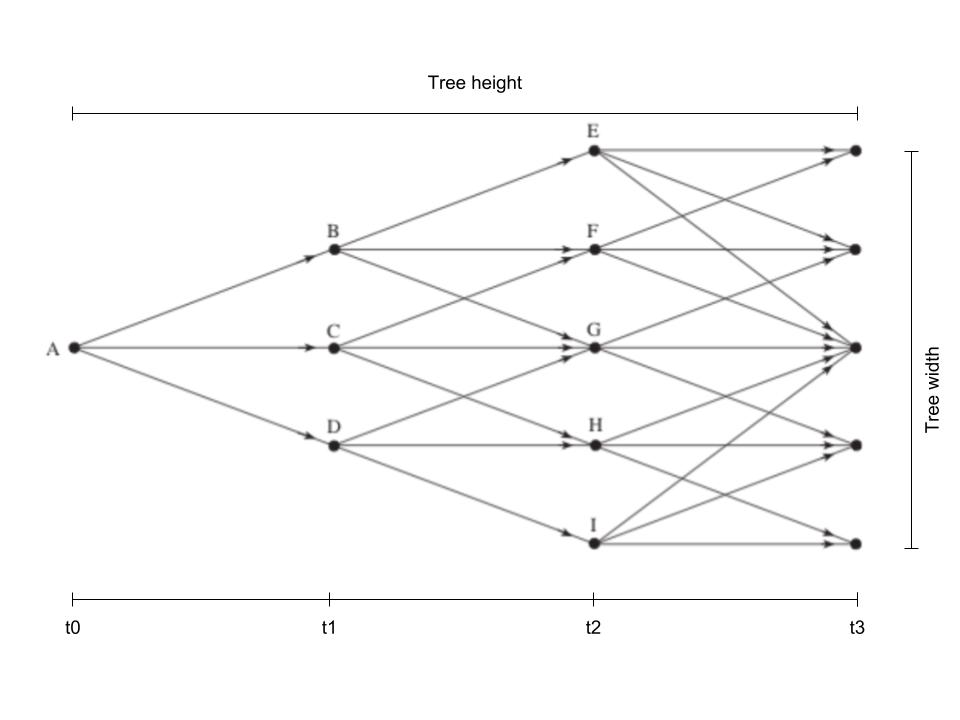
\includegraphics[width=0.8\textwidth]{img/treeconststage1wh.jpg}
	\caption{Example of a trinomial tree constructed for the hull-white one-factor model, illustrating its width and height.}
	\label{fig:intro:tree}
\end{figure}

Last, but not least we will look into inspector/executor techniques to distinguish between the performance of all parallel implementations on different data distributions and determine the most performant version for each data set. This can be done in several ways, e.g. by looking at the code first and giving a solution - known as static analysis, or by looking at the data first and then choosing the code version - known as dynamic analysis, or by doing hybrid analysis, which would be in between the two above-mentioned analysis techniques. This last point can in theory become a thesis of its own and further look into automating some or all of the actions by implementing a compiler, which could solve similar problems more efficiently later. 

% - give the high level of A solution - say what is new about our stuff compared to the related work. batch trinom-pricing is challenging due to two levels of divergence (width and height). can show the figure and briefly explain it with the tree, where width and height are shown. briefly and at high level sketch the solution in understandable terms - give the main components e.g. several versions that "make sense"; we are going to demonstrate that there is not a clear winner between them; how to choose the right version?; static analysis? - looking at the code and giving a solution; dynamic analysis? - not looking at the code; hybrid analysis? - combination of the two. analytical measure of the overhead over to divergence and on this we will choose the right version at runtime. done by inspector/executor technique. These things can generally be extracted and done automatically by a compiler in order to solve related problems.

\section{Thesis contributions}
\label{section:thesiscontributions}
The work done in this thesis will contribute by: 
\begin{itemize}
    \item analysis on how the hull-white single-factor model can be flattened
    \item multiple parallel implementations of the hull-white one-factor model in CUDA
    \item multiple parallel implementations of the hull-white one-factor model in Futhark
    \item empirical validation that validates our claims. 
    \item inspector/executor analysis on the model for further performance optimization 
\end{itemize}
	
	
% \section{Road map}
% \label{section:roadmap}
% - road map (only if the thesis ends to be too long)

% \paragraph{}
% The purpose of this thesis is to develop multiple accelerated parallel implementations of the above-mentioned pricing model using trinomial trees, aiming to achieve an optimal computation time. It will study code transformations for accelerated execution of financial instruments pricing on modern massively-parallel hardware components (involving CPUs and GPUs). Furthermore, the project will study the different performance advantages of each implementation on various data sets in order to determine which parallel techniques work best in each of the data distributions. 
% \paragraph{}

% The proof-of-concept implementation will be done sequentially with the aim for algorithm correctness rather than performance and . Correctness will be assumed as soon as the approximated results\footnote{Note that, as it will be reasoned for in section \ref{section:algorithm_and_intuition}, all implementations will be done using a numerical approach, contrary to the example in the book, which uses an analytic approach, thus the results may differ, yet should be relatively close to compare} are relatively close to the results provided in the book. The algorithm consists of the construction of trinomial trees for each entry in a data set, meaning that for every node in the tree there will be three edges - up, mid and down. This will produce trees with different widths and heights, which will ideally serve as a measure for choosing the appropriate implementation to run for each data set. While the algorithm allows computations along the width of the tree to be performed in parallel, each computation along the height of the tree requires input from the preceding nodes, hence disabling the possibility of parallel computations along the height.
% \paragraph{}
% Once a proof-of-concept is created, the next step will be concerned with a one-option per thread implementation. Here the computation of a single option is performed sequentially and multiple options are computed in parallel. While this closely resembles the previous approach, certain memory allocation difficulties arise in this implementation. These will be thoroughly described in chapter \ref{chapter:oneoptionperthread}. This method provides parallelism only over the number of options in the file, thus it can easily be observed that constructed option trees with larger heights and widths will generally take longer to compute on their threads. As it will be shown later in the report, it is possible to perform several pre-processing optimizations, which can possibly enhance the performance. The purpose of the one-option per thread implementation would be to prove the possibility of running the algorithm in parallel and showing a set of base running time results, which can be used to compare with the next implementations. In order to cope with implementation correctness, we will compare the results with the ones obtained from the sequential implementation.
% \paragraph{}
% The third step will focus on a multiple options per thread block implementation. Here more than one option can be priced in parallel, depending on their constructed tree widths. This can in theory be done in two ways - parallelism on he height of the tree, or parallelism on he width of the tree. Since the algorithm requires time steps to be computed sequentially, the possibility to parallelize on the height of the constructed trees is excluded. Hence, the multiple options per thread block approach aims at filling the block size with the option widths. E.g. if two options are present, each with width 500, they can be ran in parallel, as their total width is less than 1024 (the typical block size). This implies also that the option widths in the file must not exceed 1024. This implementation requires non-trivial design for the memory allocation, as well as introduces various difficulties in terms of data accesses inside the thread block. This will be described in more details in chapter \ref{chapter:multoptionsperthreadblock}. The purpose of the multiple options per thread block is to show that it produces speed up for at least some of the different data distributions. Similarly to the previous implementation, the correctness will be validated in relation to the sequential implementation.
% \paragraph{}
% The fourth step will be focused on a full flattening implementation, where all options will be executed in parallel. For this purpose all memory should be allocated globally, instead of using the shared memory space between the threads. This approach is similar to the multiple options per thread block, with the difference that all widths should be computed simultaneously (per time step). While full flattening provides the most parallelism out of all implementations, storing the arrays in global memory should significantly increase the running time, as global memory I/O operations are far more expensive compared to shared memory I/O. The purpose of this implementation would be to show the trade off between parallelism and memory locality, by showing that it will perform slower on larger data sets. This implementation will be described in more details in chapter \ref{chapter:fullflattening}. Once again, correctness of the implementation will be validated according to the sequential implementation.
% \paragraph{}
% Once all versions have been implemented and validated on the examples provided in the book, the thesis will look into expanding the data in attempt to cover different possible distributions and attempt to price various financial instruments. Since the algorithm performs on the widths and the heights of the constructed trees, it will be interesting to experiment both with uniformly distributed data, as well as skewed distributions, where a small portion of the input will be significantly different than the rest. This should increase the memory allocation and put the implementations to the test, in attempt to discover and fix possible errors that may occur when working with larger inputs. Data generation will be discussed in larger detail in chapter \ref{chapter:datageneration}.       
% \paragraph{}
% Last but not least, the thesis will look into tuning the model parameters in order to optimize the performance of all implementations. Benchmarking will be performed in order to compare and distinguish advantages and disadvantages over each implementation. Finally, using the knowledge obtained from the benchmarking, the thesis will attempt to apply inspector/executor techniques in order to choose the optimal approach (implementation) to run a data set with, based on the distribution of the inputted data.  The primary challenge in this step will be to discover patterns in a data set and determine its distribution. This step will be described in more details in chapter \ref{chapter:benchmarking} 




% (TODO: build our introduction around the following questions)
% % RESEARCH QUESTIONS AND APPROACH
% \section{Research questions and approach}
% This report will focus on the addressing the following research questions:
% \begin{enumerate}
%     \item What are general parallel patterns that exist in the implementation of trinomial trees for option pricing? We will approach this question by getting familiarized with the terminology and the financial background needed to tackle the problem.
%     \item How to implement the Hull-White One-Factor Model using trinomial trees to achieve optimal performance on modern parallel hardware platforms regardless of the the size and computation complexity of interest-rate options? We will try to achieve this by deriving three code versions, one for each thread divergence possibility.
%     \item Can the method be extended to more complex contracts while sustaining optimal performance? 
% \end{enumerate}
% The problem will be approached using concrete steps:
% \begin{itemize}
%     \item We will try to discriminate between code versions e.g. by creating a benchmark for various inputs, and assess which version is the best for each configuration.
%     \item We will experiment with inspector/executor techniques to determine optimal solution in terms of computation time (e.g. computing the height/width of each tree).
%     \item We will experiment with auto-tuning techniques like, e.g. OpenTuner~\footnote{http://opentuner.org/}, to help optimize various parameters of the model and reduce the execution time.
% \end{itemize}